\RequirePackage[T1]{fontenc}
\documentclass[conference]{IEEEtran}
\usepackage[T1]{fontenc}
\usepackage{mathptmx,amsmath,booktabs,graphicx,url,balance}
\graphicspath{{../results/course17/}{../out/course17/}}
\title{3DFUN AI: Single-Image 3D Reconstruction and Synthetic Depth Training}
\author{\IEEEauthorblockN{J Ganesh$^{1}$, M Jagadeshwar$^{2}$, B Varshith$^{3}$, Pranav Kashyap$^{4}$, C Sai Aravind$^{5}$}
\IEEEauthorblockA{Group 17, 3D Computer Vision, Indian Institute of Information Technology Dharwad\\
$^{1}$23BDS024, $^{2}$23BDS033, $^{3}$23BDS011, $^{4}$23BCS098, $^{5}$23BDS075\\
Correspondence: J Ganesh, \texttt{23bds024@iiitdwd.ac.in}}}
\begin{document}
\maketitle
\begin{abstract}
We built a local application that turns an object photograph into a textured triangle mesh. The outline and a pretrained depth estimate determine the thickness of a volume. We extract triangles from the zero level of its signed distance grid. On 13 synthetic reference objects, our meshes had mean Chamfer distance 0.0639 and F-score 0.148 at a 1\% threshold. Across all 25 scenes, 96\% of our runs produced closed meshes. In a separate experiment, we trained TinyDepth, a 24,369-parameter model, on rendered RGB and depth pairs. Its mean absolute error on a held-out cylinder was 0.124 normalized units, compared with 0.159 for a constant predictor. The ring example shows a limitation of the mesh method. The inferred volume fills an opening that should stay empty.
\end{abstract}
\begin{IEEEkeywords}
single-view reconstruction, monocular depth, signed distance field, synthetic training, mesh evaluation
\end{IEEEkeywords}

\section{Introduction}
An image records the appearance of surfaces that face the camera. It does not show how thick the object is or what the far side looks like. This makes reconstruction from one image useful for learning about 3D geometry: the visible boundary can look convincing even when the hidden geometry is incorrect. A silhouette constrains the support of a shape, but it cannot recover an internal cavity or an occluded handle.

3DFUN AI puts this tradeoff in a local application. A user uploads an image, sees the processing stages, inspects the mesh from different angles and exports a standard file. The engine keeps intermediate outputs such as the foreground and depth maps so a user can see whether a failure started during segmentation, depth estimation, or meshing. CPU inference gives a usable path when a discrete GPU is unavailable.

The second part of the project connects geometry, synthetic rendering, loss design and evaluation in one small training workflow. Synthetic meshes give us the camera parameters and the visible depth at each foreground pixel. This experiment produces depth and partial point clouds. The Studio uses a frozen pretrained estimator and a shape prior when it reconstructs meshes from photographs.

\section{Problem Statement}
The reconstruction input is one RGB or RGBA image of an isolated object, with no required camera measurements. The output is an object-centered triangle mesh, texture and preview. We want reasonable agreement with the silhouette and a mesh that can be exported and inspected locally. Absolute scale, backside texture and exact concave geometry are underdetermined. The coordinates in the exported model do not express physical dimensions.

For the supervised experiment each image has a foreground mask, calibrated synthetic camera and visible-surface depth. The network consumes RGB. The mask limits supervision to valid surface pixels. At inference, the supplied foreground and camera intrinsics allow us to back-project the predicted depth into a colored point cloud. This is a partial reconstruction of the visible surface.

\section{Literature Review}
Eigen \emph{et al.} \cite{eigen} combine coarse and local depth predictions and introduce a scale-invariant depth objective. Our small network uses a related log-depth term and a context branch. Depth Anything V2 \cite{depth} learns transferable cues from synthetic labels and large collections of unlabeled images. We use its frozen Small model in the Studio. The predicted relative inverse depth is useful for ranking foreground regions, but does not yield the thickness needed for a complete mesh.

U$^2$-Net \cite{u2} provides a saliency mask. This helps with isolated objects, although mistakes around thin boundaries propagate into the geometry. Curless and Levoy \cite{curless} integrate multiple aligned range maps in a volume. Our TSDF-style comparison has a single view, so it cannot exploit the overlapping scans that make range fusion valuable. A silhouette extrusion baseline keeps the outline but imposes constant thickness.

Marching Cubes \cite{cubes} converts a scalar grid to triangles. Its output depends on the sampling and the assumptions that created the grid. Taubin smoothing \cite{taubin} reduces mesh noise. TripoSR \cite{triposr} is a learned alternative that reconstructs from a single image using learned priors. It is available as an optional ONNX provider; it was not included in the three-method CPU benchmark.

\section{Objectives}
\begin{itemize}
\item Reconstruct and export a textured GLB mesh from one object image on a local machine.
\item Make the mask, depth cues, and mesh stages available for inspection.
\item Train a compact predictor from synthetic RGB and depth, and test it on a held-out shape instance.
\item Compare the mesh pipeline with two baselines and document errors on thin and concave objects.
\end{itemize}

\section{Methodology}
\subsection{Reconstruction from one image}
The input is oriented, cropped and composited on a neutral square canvas. The foreground comes from an alpha channel or U$^2$-NetP followed by mask cleanup. We scale the foreground inverse-depth values using the second and 98th percentiles, clamp to $[0,1]$, smooth the result, and optionally apply a weak left-to-right symmetry prior. Let $d(p)$ denote the resulting closeness at pixel $p\in\Omega$, where $\Omega$ is the foreground silhouette. The width $W$ of the projected object sets a thickness limit $t_{\max}=\max(t_{\min},kW)$:
\begin{equation}
t(p)=t_{\min}+(t_{\max}-t_{\min})
\operatorname{clip}_{[0,1]}\!\left(f+g\,d(p)^\gamma\right).
\end{equation}
The draft preset uses $k=0.70$, $f=0.55$, $g=0.45$, $\gamma=0.85$ and $t_{\min}=0.02$. The volume is occupied when $p\in\Omega$ and $|z|\leq t(p)/2$. Increasing $f$ gives the silhouette a stronger constant core; increasing $g$ makes depth more influential. The slab is centered on the same plane and does not model measured back-facing surfaces.

The signed distance field is the outside distance transform minus the inside transform. A Gaussian smooths it before the zero isosurface is extracted. The engine removes small components, smooths and decimates the surface, and projects the source into a texture atlas with an estimated back texture. Texture makes inspection easier but can hide geometric errors. Figure~\ref{fig:outputs} therefore includes multiple views and a difficult example.

\subsection{Synthetic data and network}
We generate two boxes, two cylinders, a cone, a sphere, an ellipsoid and a capsule. We center each mesh and divide coordinates by its largest bounding-box extent. We render each sample at eight camera poses at $96\!\times\!96$ pixels, with a focal length of $1.2$ times the image width and a depth translation of 1.8 units. Lambertian shading gives shape cues in RGB. We interpolate perspective depth from reciprocal vertex $Z$ and retain the closest fragment at a pixel. The renderer writes RGB, depth, masks, normals and camera parameters. A 16-bit PNG stores normalized depth multiplied by 1000, with zero reserved for background.

We kept all views of a mesh in one split. We used 48 training views from six meshes, eight capsule views for validation and eight cylinder views for testing. The training set included a wider cylinder, so this split tested a different instance of a familiar shape family. The packaged trainer can reuse rendered datasets, record the split and keep a chosen shape family together through an explicit mesh assignment. The results below come from the recorded CPU experiment.

TinyDepth computes 16 full-resolution feature channels. Three convolutions, including one dilated layer, form a stride-two context branch. After bilinear upsampling, context is concatenated with the original features. Two convolutions and a softplus return positive depth. For a valid foreground pixel $i$ define $r_i=\log(\hat z_i)-\log(z_i)$. The objective is
\begin{equation}
\mathcal L=\sqrt{\overline{r^2}-0.85\bar r^{\,2}}
              +\lambda_g\mathcal L_\mathrm{grad}.
\end{equation}
The gradient term averages absolute log-residual differences over valid neighbors at three scales. We run 20 epochs with AdamW, a cosine learning-rate schedule starting at 0.002, batch size 4 and seed 17. The checkpoint with lowest validation MAE is selected before test evaluation. Export verifies numerical agreement with ONNX Runtime at two input sizes and batch shapes.

\subsection{Evaluation protocol}
The recorded mesh benchmark has 13 reference meshes and 12 real image-only scenes. The three methods run three times per scene on CPU for 225 runs. Geometry uses 20,000 area-weighted surface samples on independently centered, scaled and inertia-aligned meshes. We report symmetric unsquared Chamfer distance, F-score at $\tau=0.01$ of normalized object size, and IoU of occupied surface-sample bins on a shared $64^3$ grid. The last metric describes surfaces rather than solid volumes. Closure and runtime use all scenes. Only the synthetic cases have ground truth for geometry.

For TinyDepth, we average per-image foreground MAE, RMSE, absolute relative error (AbsRel) and fraction $\delta_1$ inside the depth ratio threshold 1.25. The constant baseline uses the median of the per-image foreground medians in training. The loss ablation repeats training with the same split, seed and checkpoint rule with $\lambda_g=0$.

\begin{figure*}[!t]
\centering
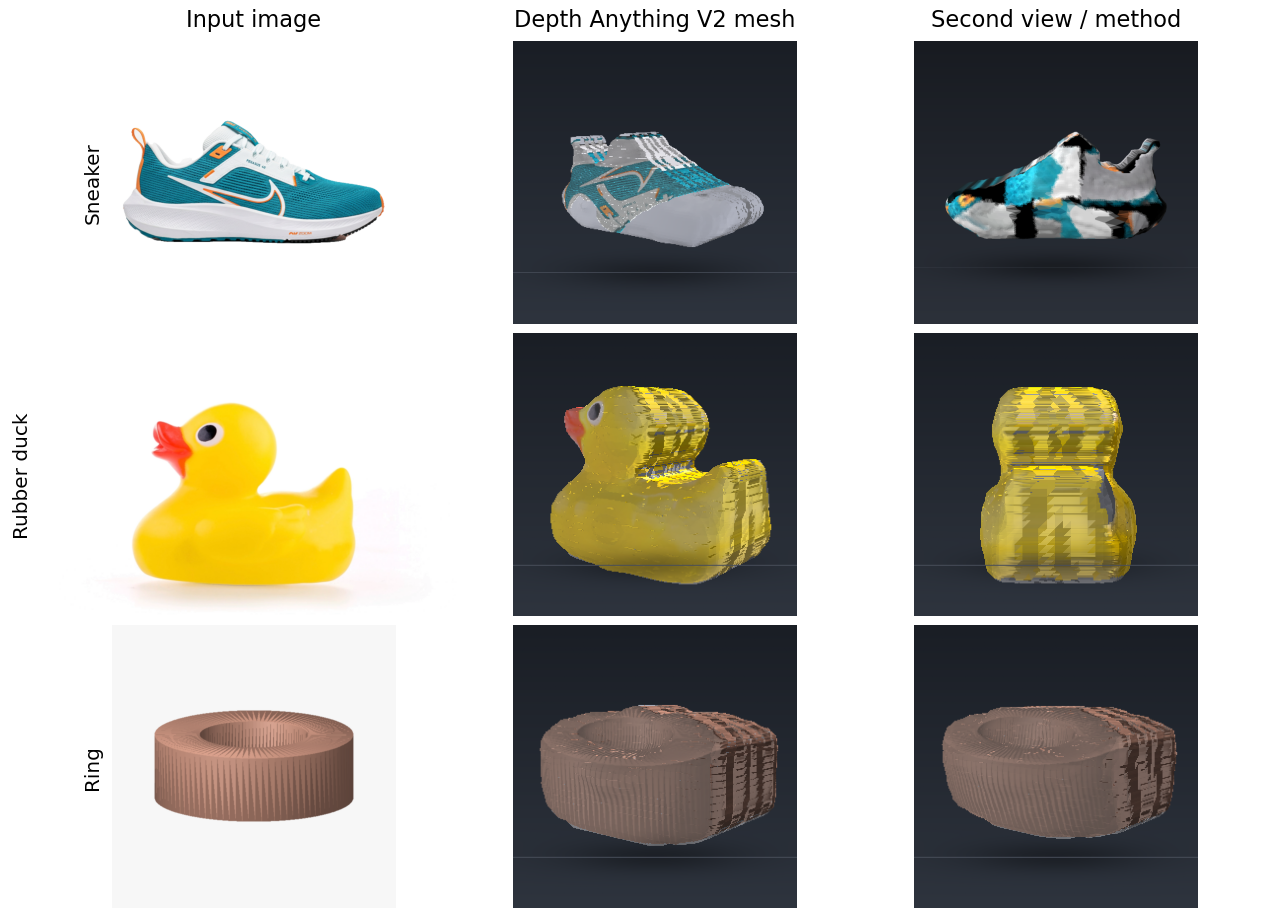
\includegraphics[width=.78\textwidth]{output_comparison.png}
\caption{Reconstructed meshes. The last column shows a second view for the sneaker and duck and the MiDaS Small result \cite{midas} for the ring. Both ring reconstructions fill the opening.}
\label{fig:outputs}
\end{figure*}

\section{Results and Discussion}
\subsection{Mesh benchmark}
Table~\ref{tab:mesh} shows that the depth-guided method had the lowest Chamfer and highest F-score of the compared methods. The absolute F-score and IoU still show a large gap to the reference surface even when the result is closed. The baselines were faster; since the implementations do different amounts of preprocessing and texture work, these timings describe the local pipelines.

\begin{table}[!t]
\caption{Recorded CPU benchmark. CD is mean Chamfer distance.}
\label{tab:mesh}
\centering\footnotesize\setlength{\tabcolsep}{4pt}
\begin{tabular}{lrrrrr}
\toprule
Method & CD $\downarrow$ & F $\uparrow$ & IoU $\uparrow$ & Closed & s\\
\midrule
Depth + SDF & .0639 & .148 & .055 & 96\% & 27.73\\
TSDF-style & .0962 & .053 & .027 & 0\% & 1.43\\
Visual hull & .0728 & .098 & .038 & 0\% & 2.13\\
\bottomrule
\end{tabular}
\end{table}

\begin{table}[!t]
\caption{Selected mesh ablations over 13 reference cases.}
\label{tab:ablation}
\centering\footnotesize
\begin{tabular}{lrrr}
\toprule
Configuration & CD $\downarrow$ & F $\uparrow$ & IoU $\uparrow$\\
\midrule
Full & .0639 & .148 & .055\\
No constant core & .1016 & .071 & .023\\
No depth term & .0811 & .112 & .041\\
Reduced thickness & .0910 & .102 & .036\\
Coarser voxel grid & .0637 & .142 & .054\\
\bottomrule
\end{tabular}
\end{table}

\subsection{Ablations and failure cases}
Removing the thickness core had the largest F-score penalty among the variants in Table~\ref{tab:ablation}. Removing the depth term was also worse. A coarser grid had comparable Chamfer and slightly lower F-score. This may be a useful resource tradeoff. The comparison uses a small fixed set of scenes.

Thin plates show why we measure both silhouette and geometry. The plate had F-score 0.023 and Chamfer 0.140 on the first run even with silhouette IoU 0.687. The ring had silhouette IoU 0.658 but F-score 0.082. The thickness prior and mask cleanup can close an opening that should stay empty. The asymmetric stairs had F-score 0.032 on the first run. Mirroring the texture does not correct these geometric errors.

We also provide a calibration program that runs pretrained depth once per scene and measures Chamfer on Marching Cubes surfaces while varying thickness, floor, exponent and SDF smoothing. The default preset remains a candidate. The program scores fit and held-out scenes separately. It measures the lower-resolution volume stage before mesh cleanup, so its scores should not be mixed with Table~\ref{tab:mesh}. In the eight-trial run, mean fit Chamfer fell from 0.0595 to 0.0511. Held-out mean Chamfer moved from 0.0951 to 0.0932, while the thin plate worsened from 0.1403 to 0.1605. This is why we keep the Studio default and report calibration separately.

\begin{figure*}[!t]
\centering
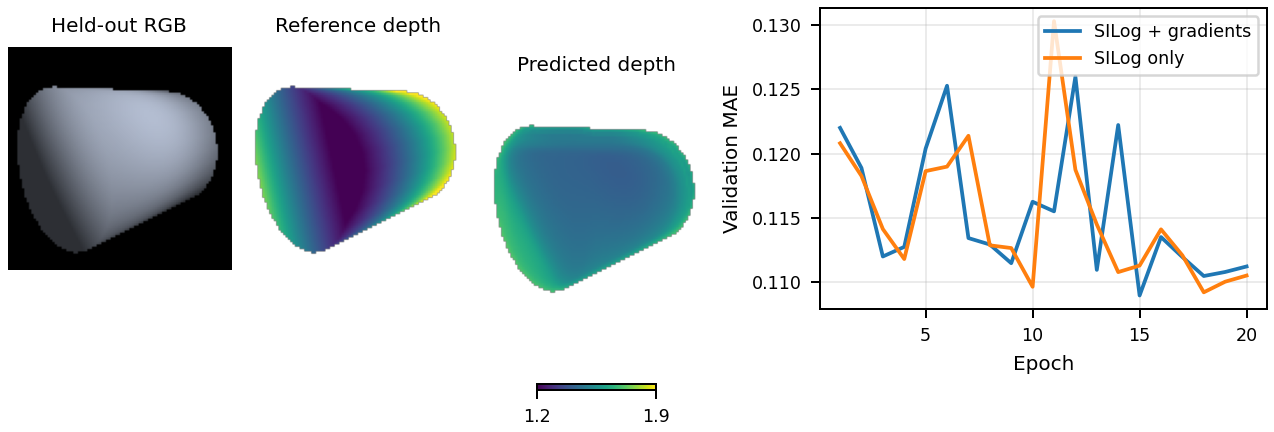
\includegraphics[width=.98\textwidth]{tinydepth_figure.png}
\caption{TinyDepth experiment. Left: a held-out cylinder render and its reference and predicted depth, on the same normalized scale. Right: validation MAE curves used for checkpoint selection.}
\label{fig:training}
\end{figure*}

\subsection{Depth experiment}
The full model reached test MAE 0.1239 compared with 0.1591 for the constant predictor, a relative reduction of about 22\% (Table~\ref{tab:depth}). Gradients modestly improved the scores over the SILog-only run. This is one seed and one test instance, so we do not infer that gradients improve other mesh families. Figure~\ref{fig:training} shows that the prediction captures some depth variation but smooths local details. The high $\delta_1$ scores partly reflect the narrow range of depths around the camera translation.

\begin{table}[!t]
\caption{TinyDepth on eight held-out cylinder views.}
\label{tab:depth}
\centering\footnotesize
\begin{tabular}{lrrrr}
\toprule
Method & MAE $\downarrow$ & RMSE $\downarrow$ & AbsRel $\downarrow$ & $\delta_1$ $\uparrow$\\
\midrule
Constant depth & .1591 & .1768 & .1185 & .949\\
SILog only & .1267 & .1449 & .0954 & .987\\
SILog + gradients & .1239 & .1411 & .0931 & .989\\
\bottomrule
\end{tabular}
\end{table}

Given predicted $Z$ and known intrinsics, we back-project a valid pixel center $(u,v)$ to $X=(u-c_x)Z/f_x$ and $Y=(c_y-v)Z/f_y$. The inference script writes the visible colored cloud to PLY so students can see how depth errors become errors in 3D. Unknown intrinsics, background segmentation and occluded surfaces fall outside that experiment. The checkpoint is separate from the pretrained estimator used by Studio.

We computed symmetric unsquared Chamfer distance and F-score in the camera frame using the same sample of up to 4,096 foreground pixels per view. At a distance threshold of 0.01 normalized units, SILog with gradients achieved Chamfer 0.0980 and F-score 0.0456 across the eight cylinder views. SILog alone reached 0.0989 and 0.0424. The constant predictor reached 0.1358 and 0.0211. The low F-scores show that few points fell within the tight threshold. The archive includes the per-view measurements. The updated pipeline can compare both loss settings using identical held-out views and export the per-mesh differences.

\balance
\section{Conclusion}
The local workflow exposes the stages of single-image mesh reconstruction and trains a small supervised depth model. In our benchmark, a depth-guided volume and constant thickness core improved geometric scores over the selected baselines. Mesh closure did not assure geometric accuracy. TinyDepth beat its constant baseline under controlled rendering conditions. A larger holdout, real depth data, and multi-view consistency checks would make the claims stronger. A representation of free space or a multi-view pipeline could address the closed ring and other thin-structure failures.

\begin{thebibliography}{8}
\bibitem{eigen} D. Eigen, C. Puhrsch, and R. Fergus, \emph{Depth map prediction from a single image using a multi-scale deep network}, Proc. NeurIPS, 2014.
\bibitem{depth} L. Yang, B. Kang, Z. Huang, Z. Zhao, X. Xu, J. Feng, and H. Zhao, \emph{Depth Anything V2}, Proc. NeurIPS, 2024.
\bibitem{u2} X. Qin \emph{et al.}, \emph{U$^2$-Net: Going deeper with nested U-structure for salient object detection}, Pattern Recognit., vol. 106, Art. no. 107404, 2020.
\bibitem{curless} B. Curless and M. Levoy, \emph{A volumetric method for building complex models from range images}, Proc. SIGGRAPH, 1996, pp. 303--312.
\bibitem{cubes} W. E. Lorensen and H. E. Cline, \emph{Marching cubes: A high resolution 3D surface construction algorithm}, Proc. SIGGRAPH, 1987, pp. 163--169.
\bibitem{taubin} G. Taubin, \emph{A signal processing approach to fair surface design}, Proc. SIGGRAPH, 1995, pp. 351--358.
\bibitem{triposr} D. Tochilkin \emph{et al.}, \emph{TripoSR: Fast 3D object reconstruction from a single image}, arXiv:2403.02151, 2024.
\bibitem{midas} R. Ranftl, K. Lasinger, D. Hafner, K. Schindler, and V. Koltun, \emph{Towards robust monocular depth estimation: Mixing datasets for zero-shot cross-dataset transfer}, arXiv:1907.01341, 2019.
\end{thebibliography}
\section*{Author Contributions}
J Ganesh and M Jagadeshwar worked on the reconstruction engine, dataset and benchmark. B Varshith and Pranav Kashyap worked on the backend, authentication and generation jobs. C Sai Aravind and B Varshith worked on the Studio, 3D viewer and gallery. All five contributed to the report and submission materials. We used AI assistance to review the scripts, report and archive.
\end{document}

